\documentclass[12pt]{article}
\usepackage[margin=1in]{geometry}
\setlength{\parindent}{0pt} % This is the set the indent length for new paragraphs, change if you want.
\setlength{\parskip}{5pt} % This sets the distance between paragraphs, which will be used anytime you have a blank line in your LaTeX code.
%\pagenumbering{gobble}
\usepackage{amsmath,amsthm,amssymb}
\usepackage{float}
\usepackage{graphicx}
\usepackage{color}
\usepackage{enumerate}
\usepackage{enumitem}
\usepackage{multicol}
\usepackage{subcaption}
\usepackage{hyperref}
\hypersetup{
    colorlinks=true,
    linkcolor=blue,
    filecolor=magenta,      
    urlcolor=cyan,
}
\usepackage{comment}
\usepackage{cancel}
\usepackage[autostyle, english=american]{csquotes}
\MakeOuterQuote{"}

%------------------------------------------ 
\begin{document}

\title{22.212 - Reactor Physics II - PSet 03} 
\author{Travis J. Labossi\`{e}re-Hickman} 
\date{}
\maketitle 

\section{Background}\label{sec:background}

The objective of this assignment was to write a Method of Characteristics (MOC) solver to find the one-group volume-averaged fluxes and the Dancoff factors for an infinite lattice of 2-D pincells as a function of moderator cross section. The pins have a radius of 0.4 cm and a pitch of 1.26 cm. In this problem, moderator is a pure absorber, and the fuel cross section is pure scatter.


\begin{figure}[h]
\centering
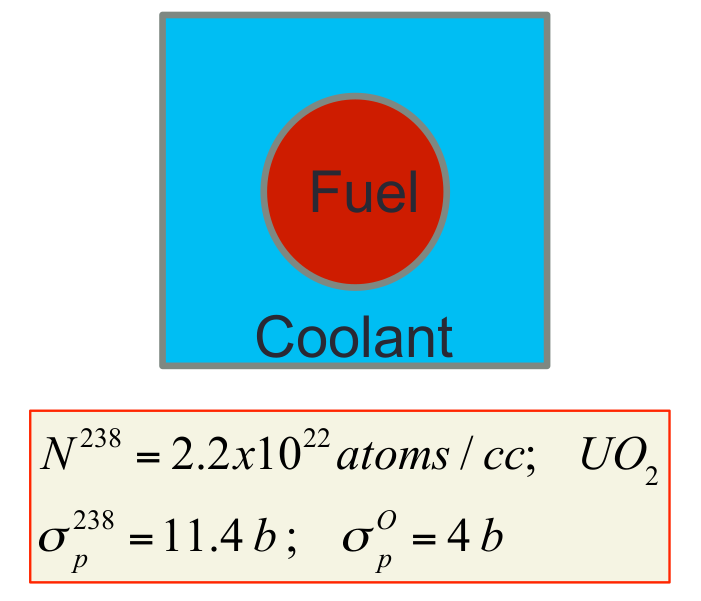
\includegraphics[width=0.67\textwidth]{figs/given.jpg}
\caption{Given data for this PSet}
\label{fig:given}
\end{figure}

A ray tracer was written for the geometry depicted in Fig.~\ref{fig:given}, and an MOC solver was written to perform the flux calculations. The source code is available on github here: \href{https://github.com/tjlaboss/moc}{github.com/tjlaboss/moc}

\newpage

\section{Methods}\label{sec:methods}

\subsection{The Method of Characteristics}\label{sec:moc}

Generally speaking, the Method of Characteristics solves the Boltzmann along "orbits," or characteristic curves, where the equation becomes an ordinary differential equation (ODE). In neutron transport, the characteristics take the form of tracks across the geometry. Integrating over a track allows the reactor physicist to solve for the angular neutron flux along that track, with the incoming flux from the edge of the geometry as the boundary condition.

\begin{figure}[h]
\centering
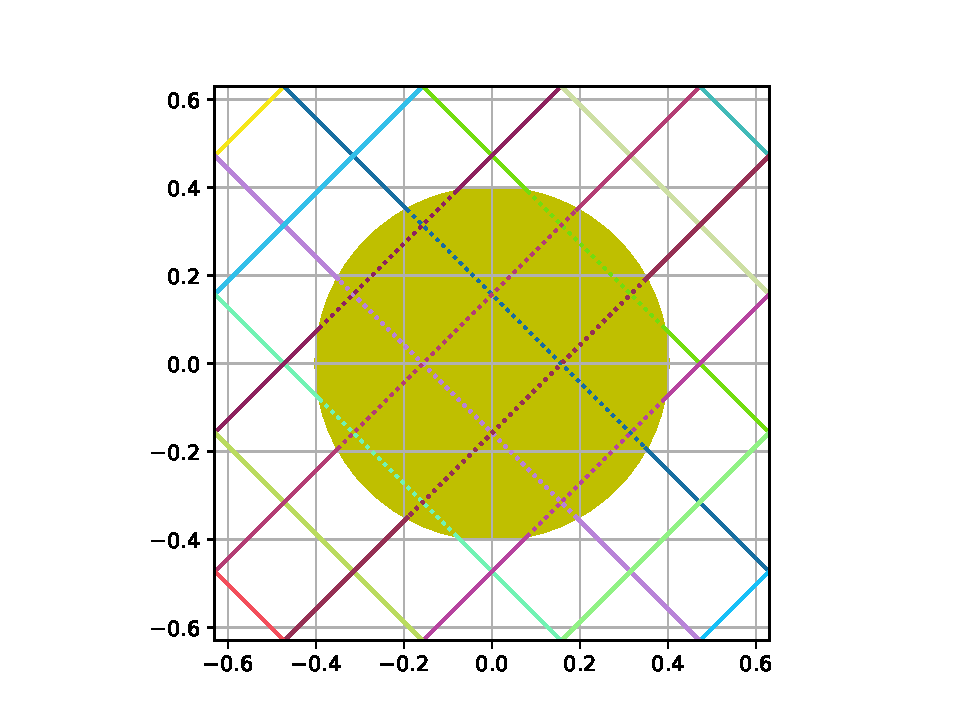
\includegraphics[width=0.67\textwidth]{figs/Tracks.pdf}
\caption{Example of tracks over a pincell geometry}
\label{fig:characteristics}
\end{figure}


\subsection{Derivation from the Neutron Transport Equation}\label{sec:derivation}

The Boltzmann neutron transport equation is

\begin{gather}\label{eq:nte}
\mathbf{\hat{\Omega}}\cdot\nabla \psi(\vec{r},E,{\hat{\Omega}}) +
\Sigma_{t} (\vec{r},E) \psi(\vec{r},E,\hat{\Omega}) = \cr
\frac{\chi \left(\vec{r}, E \right)}{4\pi} \frac{1}{k_\text{eff}}
\int\limits_0^{\infty} \int\limits_{4\pi}
\nu\Sigma_f \left(\vec{r}, E^{\prime}, \hat{\Omega} \right)
\phi \left( \vec{r}, E^{\prime}, \hat{\Omega} \right) d\Omega dE^{\prime}  + 
\int\limits^{\infty}_{0} \int\limits_{4\pi}
\Sigma_s(\vec{r}, E^\prime \rightarrow E,  \hat{\Omega}^\prime \rightarrow \hat{\Omega})
\phi(\vec{r},E^\prime, \hat{\Omega}^\prime) d\hat{\Omega}^\prime dE^\prime 
\end{gather}

Integrate Eq.~\ref{eq:nte} over all energies to get the one-group formulation. Replace the RHS of the transport equation with a single term, $Q^\prime (\vec{r}, \hat{\Omega})$ for simplicity.

\begin{gather}\label{eq:onegroup}
\mathbf{\hat{\Omega}}\cdot\nabla \psi(\vec{r},\hat{\Omega}) +
\Sigma_{t} (\vec{r}) \psi(\vec{r},\hat{\Omega}) = 
Q^\prime (\vec{r}, \hat{\Omega})
\end{gather}

To get the neutron transport equation in characteristics form, parameterize the spatial variable $\vec{r}$ in terms of angle and parameter $s$. In two dimensions,

\begin{equation}\label{eq:parametr}
\vec{r} = 
\left\{\begin{matrix}
x(s) \\
y(s) 
\end{matrix} \right\} = 
\left\{\begin{matrix}
x_0 + \mathbf{\Omega_x} s \\ 
y_0 + \mathbf{\Omega_y} s
\end{matrix} \right.
\end{equation}

...where $x_0$ and $y_0$ are the starting coordinates of the characteristic.
The gradient operator $\nabla$ is then replaced with $d/ds$. Parameterizing Eq.~\ref{eq:onegroup},

\begin{gather}\label{eq:parameterized}
\frac{d}{ds} \psi(s,\hat{\Omega}) +
\Sigma_{t} (s) \psi(s,\hat{\Omega}) = 
Q^\prime (s, \hat{\Omega})
\end{gather}

Now we have an ODE, as discussed in Section~\ref{sec:moc}. Eq.~\ref{eq:parameterized} can be solved along any track $k$ by means of an integrating factor--in this case,
$\exp\left(-\int\limits_0^s \Sigma_t (s^\prime) ds^\prime \right)$

\begin{equation}\label{eq:integatingfactor}
\psi(s, \hat{\Omega}) = 
\psi(x_0, y_0, \hat{\Omega}) e^{-\int\limits_0^s \Sigma_t (s^\prime) ds^\prime} + 
\int\limits_0^s 
Q^\prime (s^\prime, \hat{\Omega}^\prime)
e^{-\int\limits_0^{s^\prime} \Sigma_t (s^{\prime\prime}) ds^{\prime\prime}} ds^\prime
\end{equation}

The source term is getting quite messy. Fortunately, the flat source approximation comes to our rescue. Divide the geometry into a number of Flat Source Regions (FSRs), each with a constant, isotropic $Q_i$. Within each FSR, the cross sections are constant, such that $\Sigma_t (s^\prime) = \Sigma_{t,i}$ ; then, the integral evaluates to just $s \Sigma_{t,i}$. Along a given track $k$ through Flat Source Region $i$,

\begin{equation}\label{eq:fsr2}
\psi_{k,i}(s, \hat{\Omega}) = 
\psi_{k,i}(x_0, y_0, \hat{\Omega}) e^{-s \Sigma_{t,i}} + 
\frac{Q_i}{\Sigma_{t,i}}
\left(1 - e^{-s \Sigma_{t,i}} \right)
\end{equation}

Let $s_0$ represent the ordinate on the edge of the FSR, and rearrange the equation. 

\begin{equation}\label{eq:deltapsi}
\Delta \psi_{k,i} = 
\psi_{k,i}(s, \hat{\Omega}) - \psi_{k,i}(s_0, \hat{\Omega}) = 
\left( \psi_{k,i}(s_0, \hat{\Omega}) - \frac{Q_i}{\Sigma_{t,i}} \right)
\left( 1 - e^{-s \Sigma_{t,i}} \right)
\end{equation}

Eq.~\ref{eq:deltapsi} can be discretized in terms of angle. Let $a$ represent the index of the azimuthal angle $\varphi$, and $p$ of the polar angle $\theta$. Each track is necessarily at one discrete azimuthal angle. Conversely, in two dimensions, tracks with different polar angles $\theta$ are identical if they have the same $\varphi$. Applying this discrete ordinates approximation,

\begin{equation}\label{eq:discord}
\Delta \psi_{a,k,i,p} = 
\psi_{a,k,i,p}(s) - \psi_{a,k,i,p}(s_0) = 
\left( \psi_{a,k,i,p}(s_0) - \frac{Q_i}{\Sigma_{t,i}} \right)
\left( 1 - e^{-s \Sigma_{t,i}} \right)
\end{equation}


\subsection{Scalar Flux and Quadrature}\label{sec:quad}

In order to find the scalar flux in a region, it is necessary to integrate $\psi({\hat{\Omega}})$ over all angles. Under the discrete ordinates approximation, this integral is replaced with a summation over a finite number of polar and azimuthal angles.

\begin{equation}\label{eq:summation}
\phi_{i} \propto  
\int\limits_{4\pi} \psi_{i}({\hat{\Omega}}) d\Omega \approx 
4\pi \sum\limits_a \sum\limits_p w_a w_p \sin(\theta_p) \psi_{a,i,p}
\end{equation}

The azimuthal and polar weights ($w_p$ and $w_a$) and angles are obtained from a quadrature set. Derivation of particular quadratures can be a mathematically intense topic and is beyond the scope of this report. For the purposes of this problem set, decoupled azimuthal and polar quadratures have been taken from OpenMOC or the available literature as an input.

It is also necessary to take a weighted average over all track segments in a region in order to accurately calculate the scalar flux. Let letting $s_{k,i}$ represent a segment along track $k$ through FSR $i$. The average angular flux over the segment is

\begin{equation}\label{eq:segmentaverage}
\overline{\psi}_{k,i} = \frac{1}{s_{k,i}} 
\int\limits_{s_0}^{s_0 + s_{k,i}} \psi_{k, i}(s) ds
\end{equation}

where $\psi_{k, i}(s)$ is expressed by Eq.~\ref{eq:fsr2}. The result of the integral is below.

\begin{equation}\label{eq:segmentintegral}
\overline{\psi}_{k,i} = \frac{1}{s_{k,i} \Sigma_{t,i}}  \left[
\psi_{k,i}(s_0) \left(1 - e^{-s_{k,i} \Sigma_{t,i}}\right) + 
s_{k,i} Q_i \left(1 - 
\frac{1}{s_{k,i} \Sigma_{t,i}} e^{-s \Sigma_{t,i}} \right)
\right] 
\end{equation}

Since amoung of spacing between parallel tracks can vary by azimuthal angle, we must weight by the effective track width $w_k$. The limit of $s_{k,i} w_k$, as the number of tracks $N_K$ approaches infinity (and $w_k$ approaches 0), is equal to the area of the FSR.

\begin{equation}\label{eq:area}
\lim\limits_{N_K \to \infty} \sum\limits_k^{N_K} w_k s_{k,i} = A_i
\end{equation}

Applied to average angular flux,

\begin{equation}\label{eq:wkski}
\overline{\psi}_i \approx 
\sum\limits_k \frac{1}{A_i} w_k s_{k,i} \overline{\psi}_{k,i}
\end{equation}

So, summing each $\overline{\psi}_{a,k,i,p}$ over all tracks, segments, angles, and the corresponding weights to each, we get an approximate expression for the average scalar flux. Simplifying the equation using Eq.~\ref{eq:deltapsi}, we arrive at an expression for the scalar flux in each flat source region.

\begin{equation}\label{eq:scalarflux}
\overline{\phi}_{i} \approx \frac{4\pi}{\Sigma_{t,i}} \left[
Q_i + \frac{1}{A_i}
\sum\limits_a \sum\limits_k \sum\limits_p
w_a w_k w_p \sin(\theta_p)
\Delta\psi_{a,k,i,p} \right]
\end{equation}


\subsubsection{Azimuthal Angle Quadrature}\label{sec:azimuthal}

Due to quadrant symmetry, azimuthal angles are available in increments of 4. The set of weights calculated in Eq.~\ref{eq:azimuthal} is shown for Quadrant 1, and applies for angles in the other 3 quadrants when they are reflected across the appropriate axes. The sum of the weights in each quadrant is 0.25.

Azimuthal angles appear in approximately equal increments. The exact values of $\varphi$ are dependent upon the problem geometry. This is described further in Section~\ref{sec:trackgeneratorangles}.

According to the OpenMOC documentation, "The azimuthal angle quadrature set is computed based on the fraction of azimuthal angular space `owned' by each azimuthal angle." 

\begin{align}\label{eq:azimuthal}
w_1 &= \frac{1}{4\pi} \left[ \varphi_1 + \varphi_2 \right]
\cr
w_a &= \frac{1}{4\pi} \left[ \varphi_{a+1} - \varphi_{a-1} \right] 
 \hspace{24pt}(\text{for } 1 < a < N)
\cr
w_N &= \frac{1}{4\pi} \left[ \pi - \phi_{N-1} - \varphi_N \right]
\end{align}

\subsubsection{Polar Angle Quadrature}\label{sec:polar}

An arbitrary number of polar angles are available, although generally 1-3 are used. Note that $\theta$ is measured relative to the $z$-axis.

Because polar weights are always used with the sines of their respective angles, the \texttt{Quadrature()} class in the code always stores an array of $w_p \sin(\theta_p)$ in place of $w_p$.

\textbf{Equal Angle}

The Equal Angle polar quadrature divides the polar domain $[0, \pi/2]$ into $N$ equal angles. The boundaries of the angles are:

\begin{equation}\label{eq:equalboundaries}
\beta_p = \beta_{p-1}  + \frac{\pi}{N}
\end{equation}

...where $\beta_0 = 0$. These are used to calculate the angles themselves.

\begin{equation}\label{eq:equalangles}
\theta_p = \cos^{-1} \left( \frac{\cos(\beta_p) + \cos(\beta_{p-1})}{2} \right)
\end{equation}

The weights are 

\begin{equation}\label{eq:equalweights}
w_p = \cos(\theta_{p-1}) - \cos(\theta_p)
\end{equation}

\textbf{Leonard's Optimum}

Leonard's Optimum (LO) is another quadrature set created for MOC. Tabulated angles and weights for LO 1-3 are in Fig.~\ref{fig:tylo}.

\textbf{Tabuchi-Yamamoto}

The Tabuchi-Yamamoto (TY) quadrature set has shown excellent performance in MOC calculations. 
It "is derived to minimize the approximation error for the Bickley function in MOC."\footnote{Yamamoto, Tabuchi, Sugimara, Ushio, \& Mori, \textit{Derivation of Optimum Polar Angle Quadrature Set for the Method of Characteristics Based on Approximation Error for the Bickley Function}}. Angles and weights for TY and LO quadratures of up to order 3 provided by this reference are reproduced below.

\begin{figure}[h]
\centering
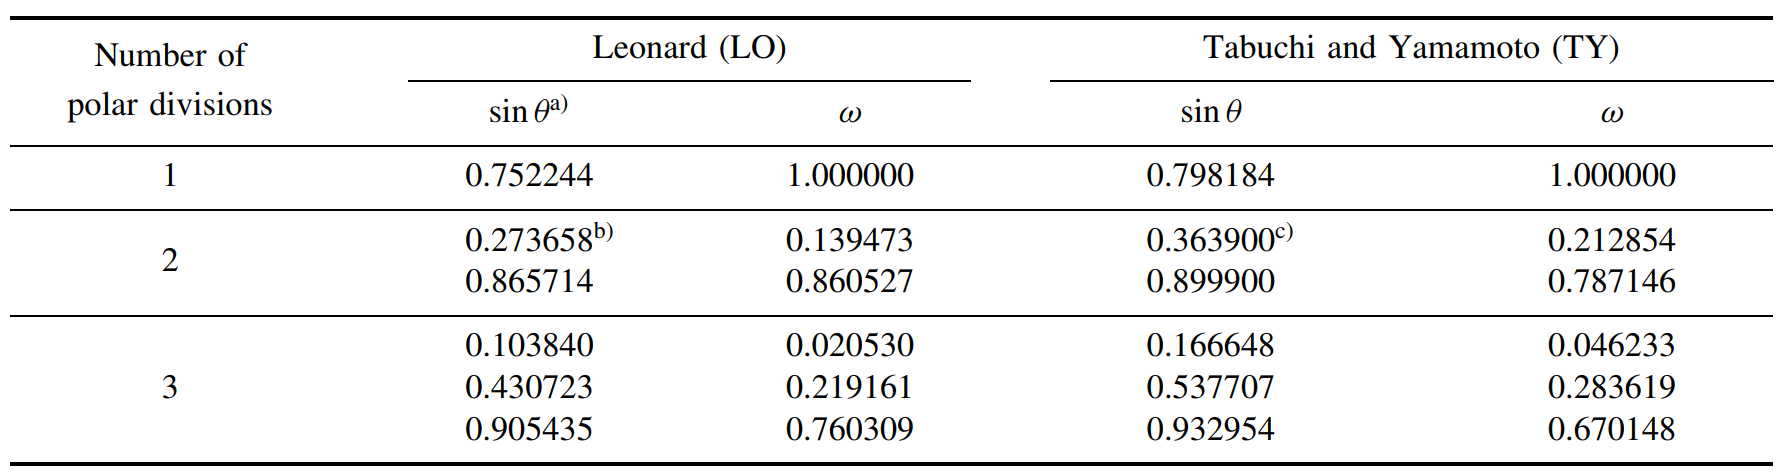
\includegraphics[width=\textwidth]{figs/TabuchiTable.png}
\caption{Polar quadrature for LO and TY}
\label{fig:tylo}
\end{figure}


\subsection{Track Generation}\label{sec:trackgenerator}

In order to apply reflective boundary conditions, it is necessary for tracks to form complete cycles over the geometry. Most geometries will require a slight adjustment to the angular distribution and track spacing in order for tracks to line up with their reflections at the boundary. The following method, adapted from Shaner et. al.,\footnote{Shaner, Gunow, Forget, Smith, \textit{Theoretical Analysis of Track Generation in 3D Method of Characteristics}} produces complete cycles of tracks.

\subsubsection{Azimuthal Angle Correction}\label{sec:trackgeneratorangles}

Let $n$ be the number of distinct track directions, provided by ther user. This corresponds to half the total number of azimuthal angles, as any angle $\vartheta $ will be along the same track as the angle $\vartheta + 180^\circ$. For index $a$ in $\left[0, n-1\right]$, we get $n$ angles in the first quadrant:

\begin{equation}\label{eq:targetn}
\vartheta = \frac{\pi}{n} \left( a + \frac{1}{2} \right)
\end{equation}

The user also specifies the desired track spacing between parallel tracks, $\delta_t$ (cm). For a given $\delta_t$, each set of angles $a$ will result in a determined number of reflection sites on each boundary, according to Eq.~\ref{eq:nxny}.

\begin{align}\label{eq:nxny}
nx_a &= \frac{\Delta x}{\delta_t} \left| \sin(\vartheta _a) \right|
\cr
ny_a &= \frac{\Delta y}{\delta_t} \left| \cos(\vartheta _a) \right|
\end{align}

...where $\Delta x$ and $\Delta y$ are the total width and height of the domain. For the purposes of our problem, an infinite lattice of pincells, these correspond to the pin pitch.

With the number of sites on each boundary known, it is trivial to calculate the $x$ and $y$ spacing of tracks on the boundary:

\begin{align}\label{eq:delxdely}
\delta x_a &= \frac{\Delta x}{nx_a}
\cr
\delta y_a &= \frac{\Delta y}{ny_a}
\end{align}

From these, we get the corrected azimuthal angles for our geometry:

\begin{equation}\label{eq:varphi}
\varphi_a = \tan^{-1}\left( \frac{\delta y_a}{\delta x_a} \right)
\end{equation}

And its second-quadrant reflection:

\begin{equation}\label{eq:ihprav}
\hat{\varphi}_a = \pi - \varphi_a
\end{equation}

Finally, we calculate the corrected azimuthal track spacing $\delta_\varphi$. This is the spacing which corresponds to the effective track width $w_k$ used in Eqs.~\ref{eq:area}--\ref{eq:scalarflux}.

\begin{equation}\label{eq:deltavarphi}
\delta_{\varphi,a} = \delta x_a \sin(\varphi_a) = \delta y_a \cos(\varphi_a)
\end{equation}


\subsubsection{Track Reflection}\label{sec:reflection}

Given the number of tracks (Eq.~\ref{eq:nxny}) and their spacing on the boundary (Eq.~\ref{eq:delxdely}), the track generator must lay down a complete set of cyclic tracks for each azimuthal angle set.

To accomplish this, the generator begins at one site along the -$x$ boundary. Knowing the angle $\varphi_a$, it is possible to trace a ray to the next boundary, a procedure which is described in Section~\ref{sec:raytracing}. Once the boundary is reached, the indices of the starting and ending sites are stored to the \texttt{Ray()} object. Then, a new ray at angle $\hat{\varphi}_a$ is spawned at the coordinates where the first ray ended, and it likewise traced to the next boundary. This process is repeated until the tracks return to within numerical tolerance of the starting coordinates.


    \begin{figure}[H]
        \centering
        \begin{subfigure}[b]{0.45\textwidth}
            \centering
            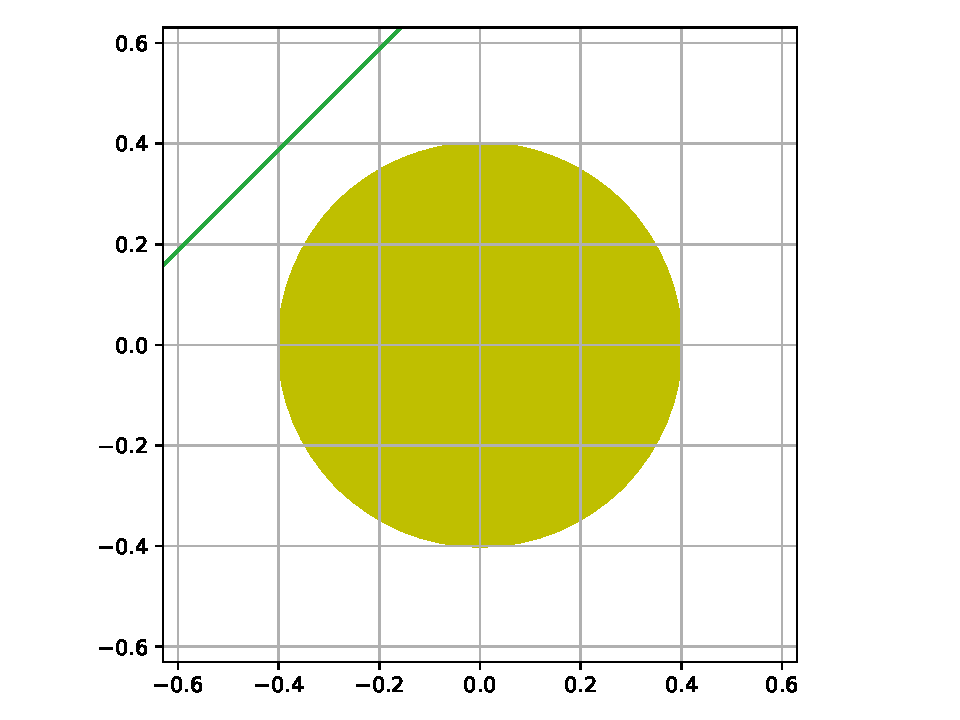
\includegraphics[width=\textwidth]{figs/Cyc1.pdf}
            \caption{Track 0 $\rightarrow$ 1}
        \end{subfigure}
        \quad
        \begin{subfigure}[b]{0.45\textwidth}  
            \centering 
            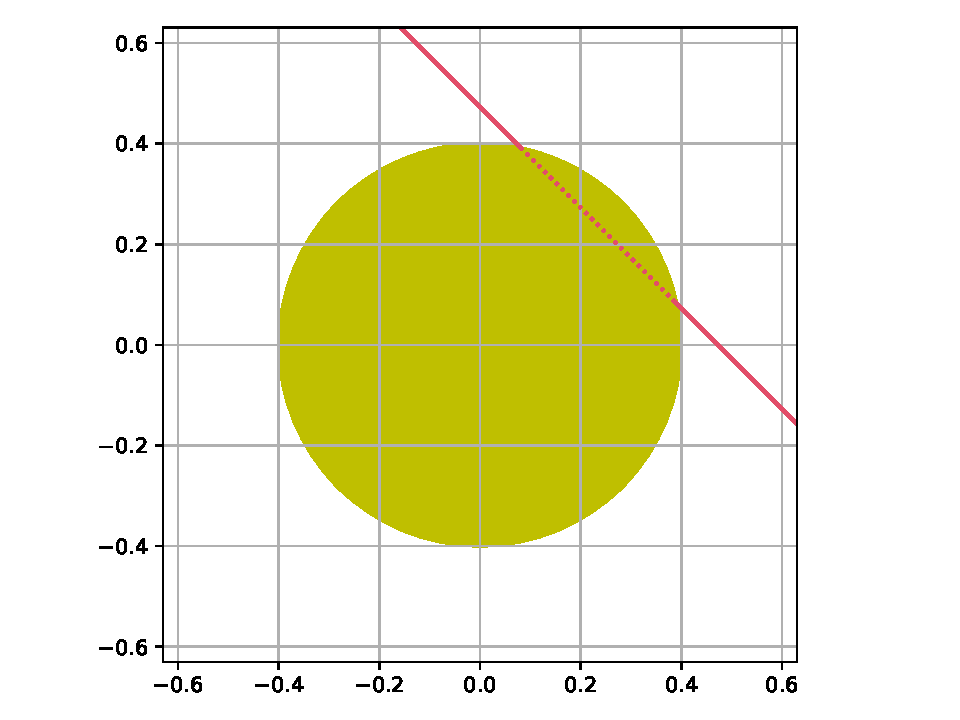
\includegraphics[width=\textwidth]{figs/Cyc2.pdf}
            \caption{Track 1 $\rightarrow$ 2}
        \end{subfigure}
        \vskip\baselineskip
        \begin{subfigure}[b]{0.45\textwidth}   
            \centering 
            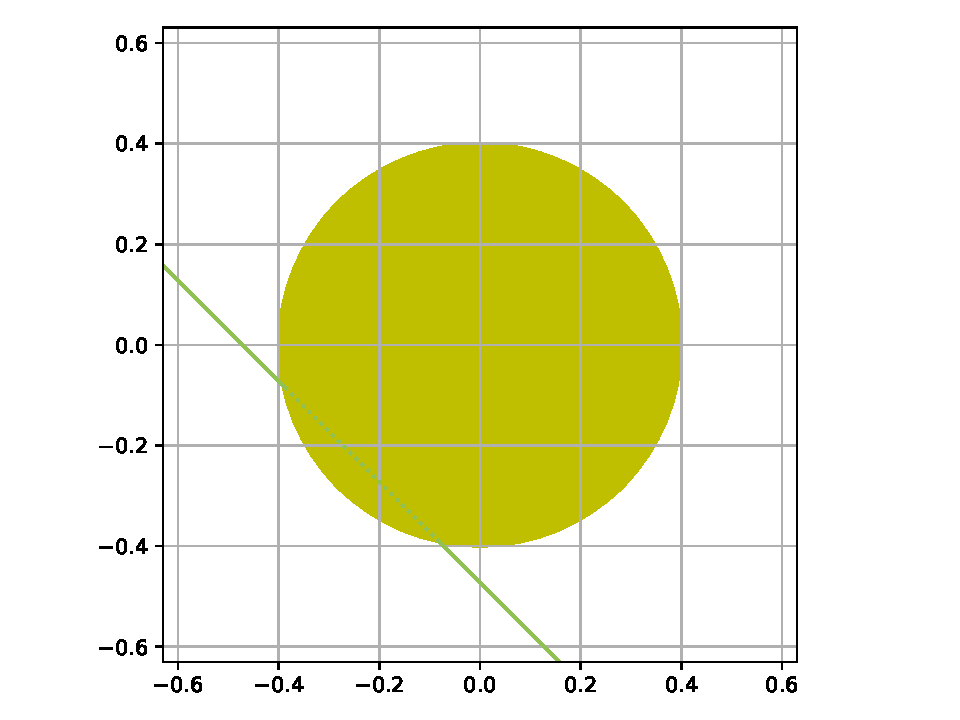
\includegraphics[width=\textwidth]{figs/Cyc4.pdf}
            \caption{Track 3 $\rightarrow$ 0}
        \end{subfigure}
        \quad
        \begin{subfigure}[b]{0.45\textwidth}   
            \centering 
            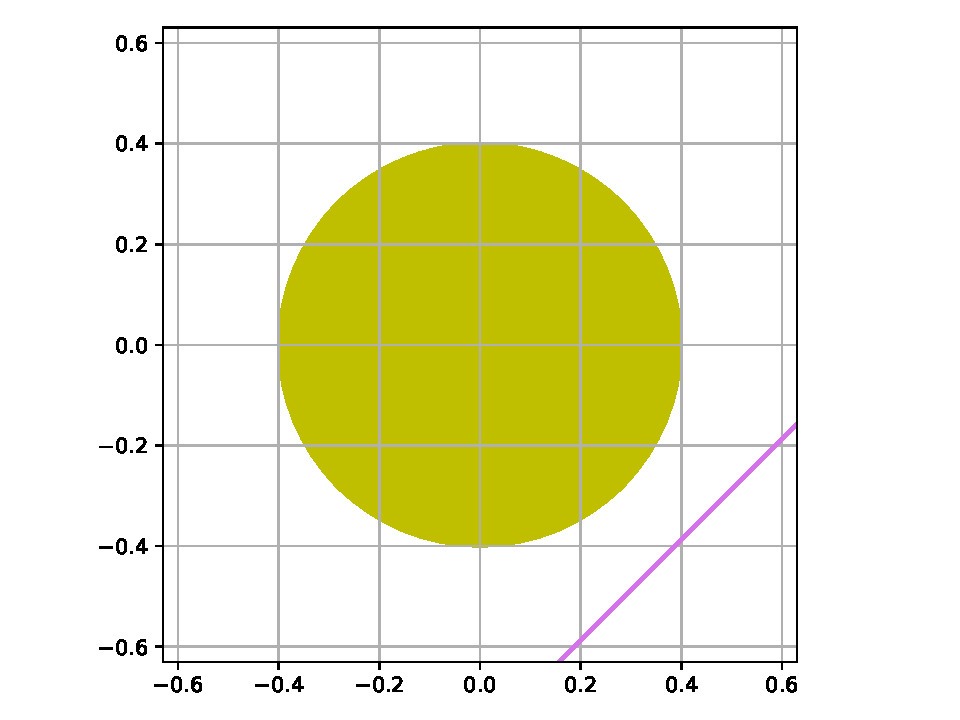
\includegraphics[width=\textwidth]{figs/Cyc3.pdf}
            \caption{Track 2 $\rightarrow$ 3}
        \end{subfigure}
        \caption{A set of tracks over one cycle}
        \label{fig:fourtracks}
    \end{figure}

\begin{figure}[h]
\centering
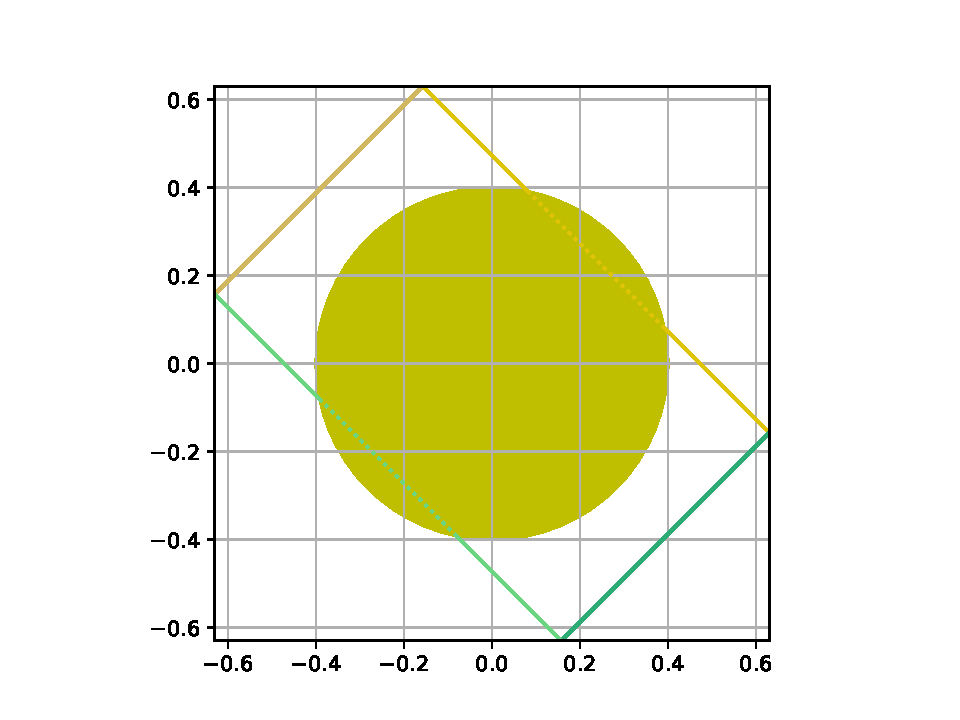
\includegraphics[width=0.55\textwidth]{figs/Cyc0.pdf}
\caption{The four tracks together}
\label{fig:cycletracks}
\end{figure}

\newpage

At certain angles (e.g., $45^\circ$, as depicted in Figs.~\ref{fig:fourtracks} and \ref{fig:cycletracks}), a complete cycle is formed before all necessary tracks have been laid. In this event, the track generator moves to the next site on the boundary which has not been used yet. This is depicted below in Fig.~\ref{fig:fourcycles}.

   \begin{figure}[H]
        \centering
        \begin{subfigure}[b]{0.45\textwidth}
            \centering
            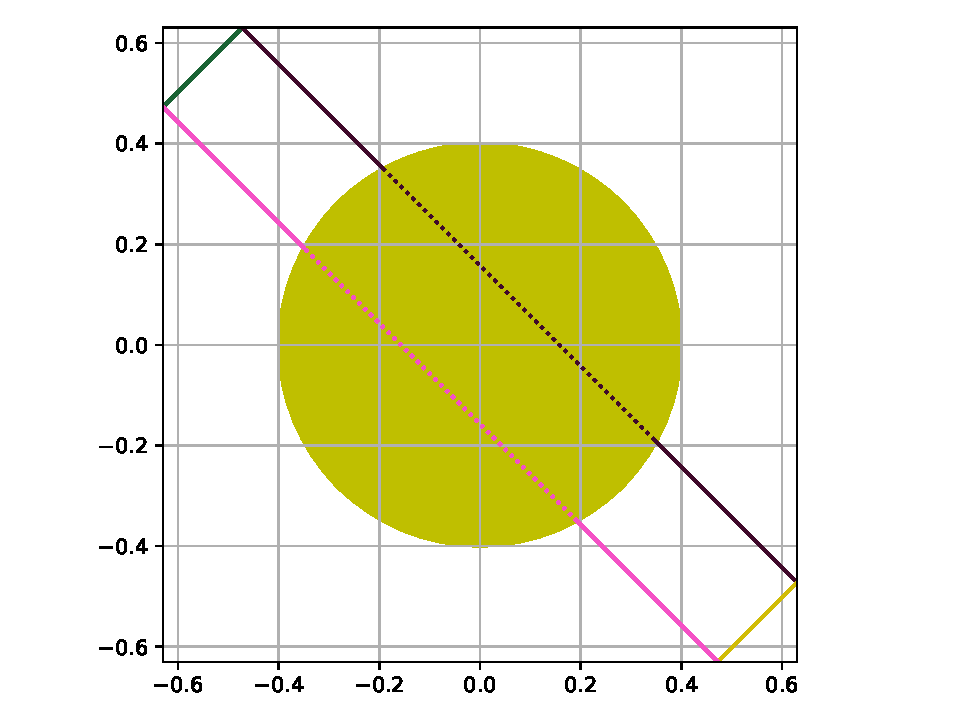
\includegraphics[width=\textwidth]{figs/Ninety1.pdf}
        \end{subfigure}
        \quad
        \begin{subfigure}[b]{0.45\textwidth}  
            \centering 
            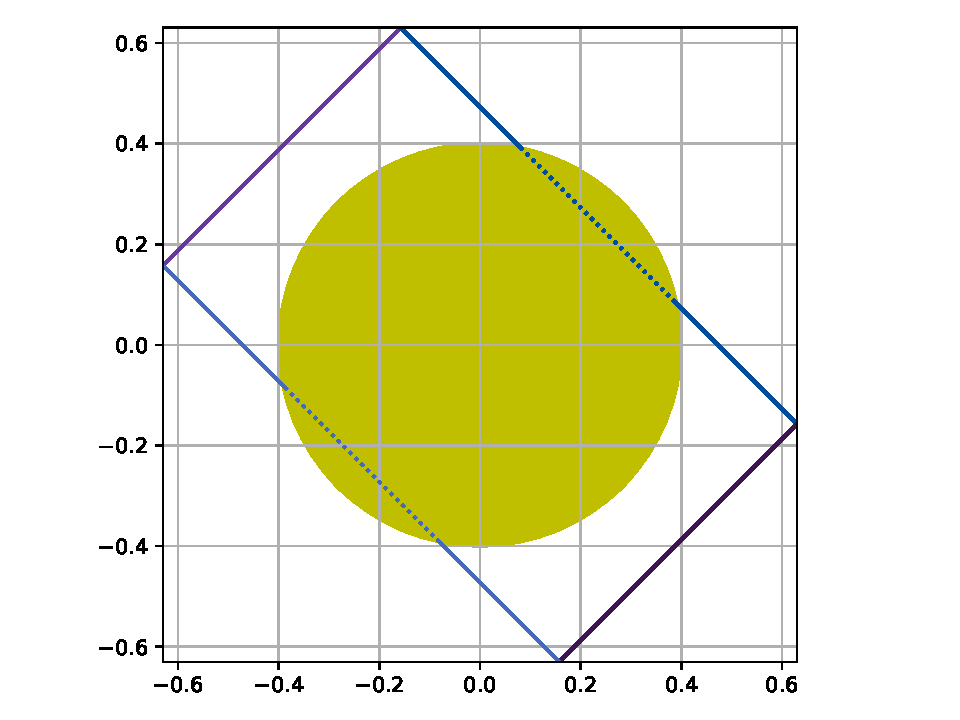
\includegraphics[width=\textwidth]{figs/Ninety2.pdf}
        \end{subfigure}
        \vskip\baselineskip
        \begin{subfigure}[b]{0.45\textwidth}   
            \centering 
            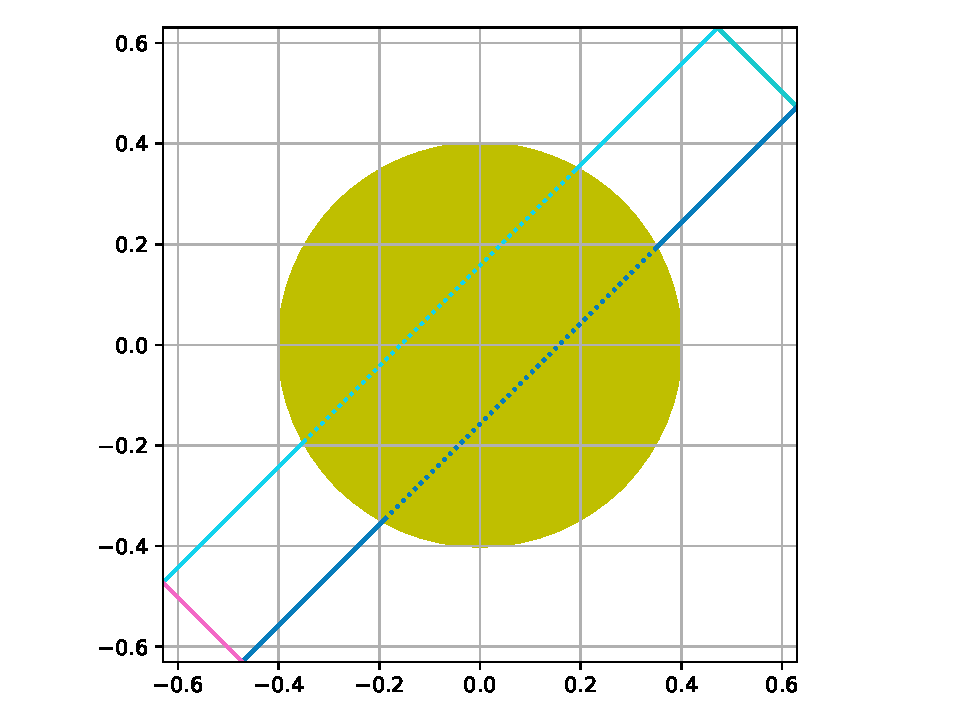
\includegraphics[width=\textwidth]{figs/Ninety4.pdf}
        \end{subfigure}
        \quad
        \begin{subfigure}[b]{0.45\textwidth}   
            \centering 
            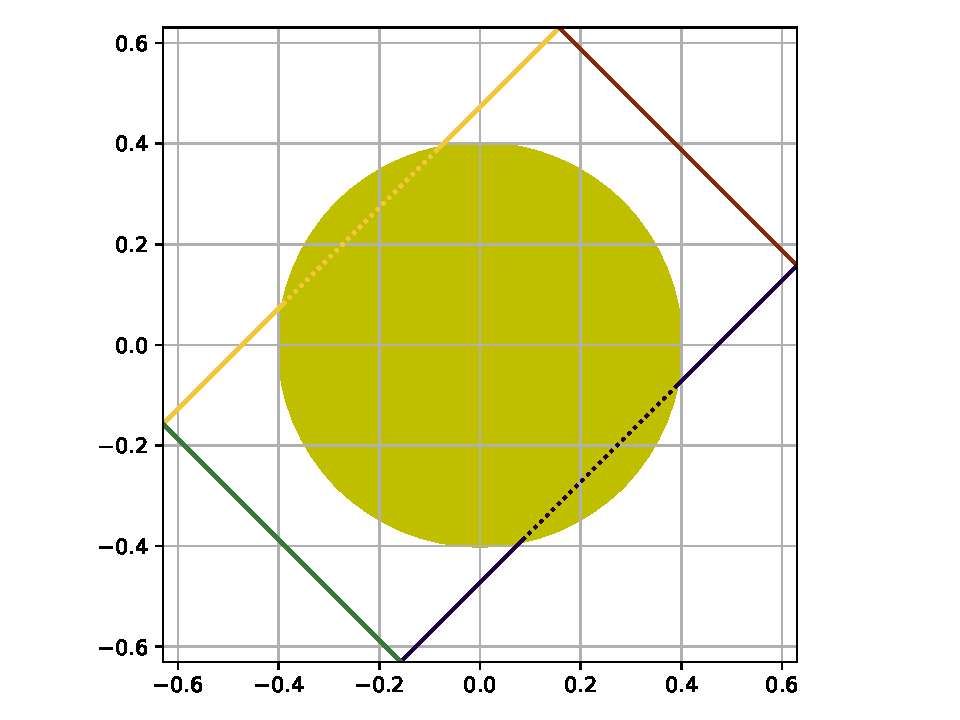
\includegraphics[width=\textwidth]{figs/Ninety3.pdf}
        \end{subfigure}
        \caption{Complete set of tracks for one angle}
        \label{fig:fourcycles}
    \end{figure}

However, most angles produce complete sets of tracks in one cycle, as seen in Fig.~\ref{fig:twocycles}.

   \begin{figure}[H]
        \centering
        \begin{subfigure}[b]{0.45\textwidth}
            \centering
            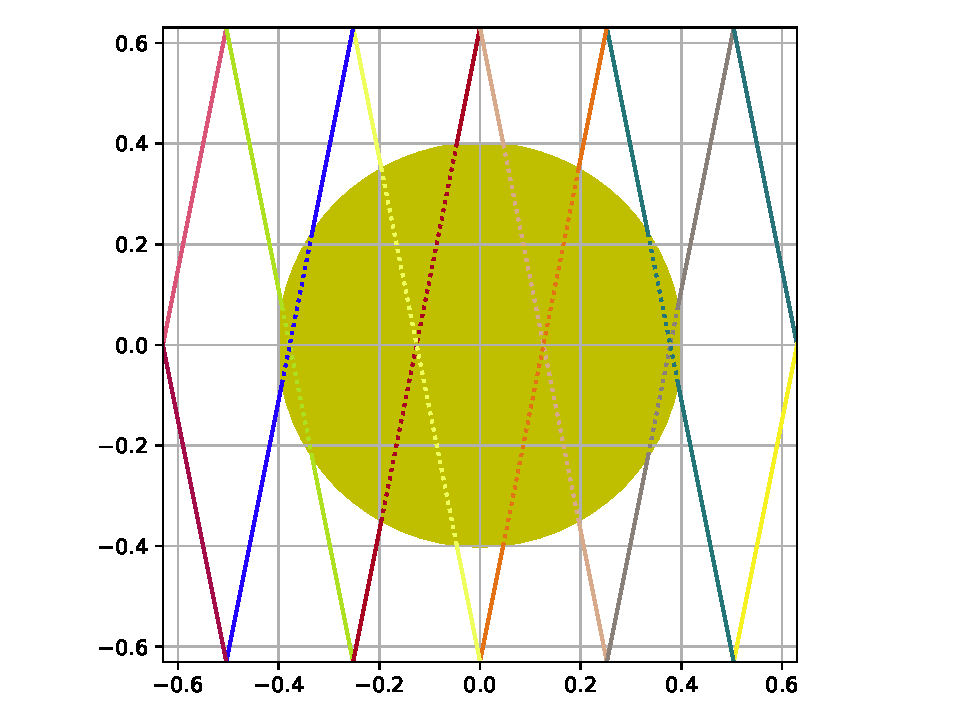
\includegraphics[width=\textwidth]{figs/Ang3.pdf}
        \end{subfigure}
        \quad
        \begin{subfigure}[b]{0.45\textwidth}  
            \centering 
            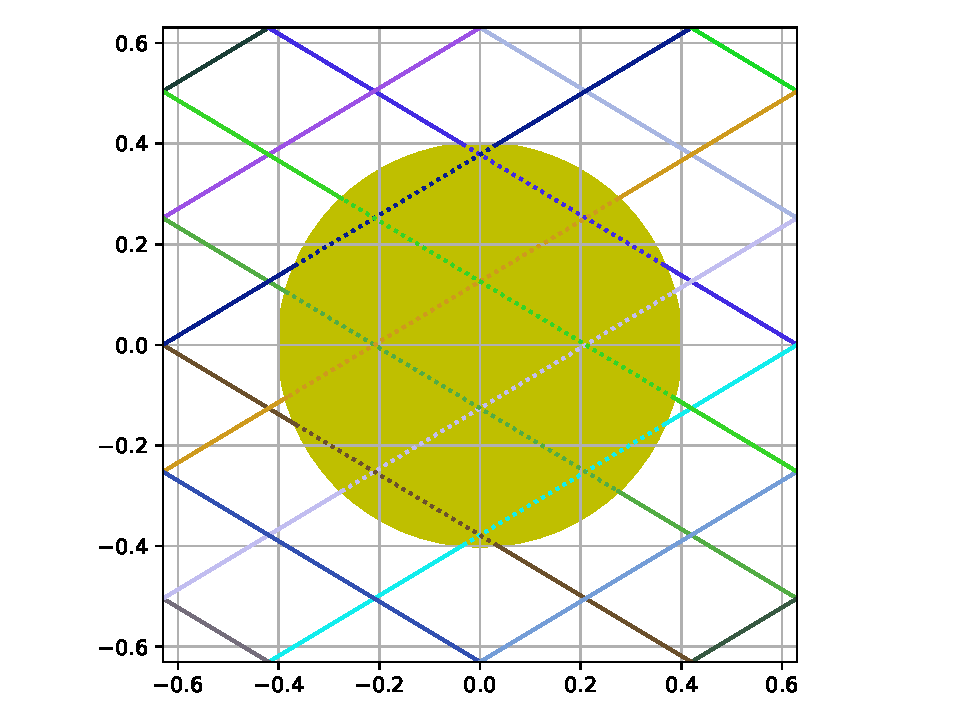
\includegraphics[width=\textwidth]{figs/Ang1.pdf}
        \end{subfigure}
        \caption{Complete sets of tracks for two angles, each over one cycle}
        \label{fig:twocycles}
    \end{figure}
    
\newpage

\subsection{Ray Tracing}\label{sec:raytracing}

Developing the ray tracing algorithm was the most challenging portion of this project. Due to the complexity of developing a general ray tracer, one was written for the specific geometry used in this problem set: a single cylindrical fuel pin with a square pitch. 

Consider the ray below: 

\begin{figure}[h]
\centering
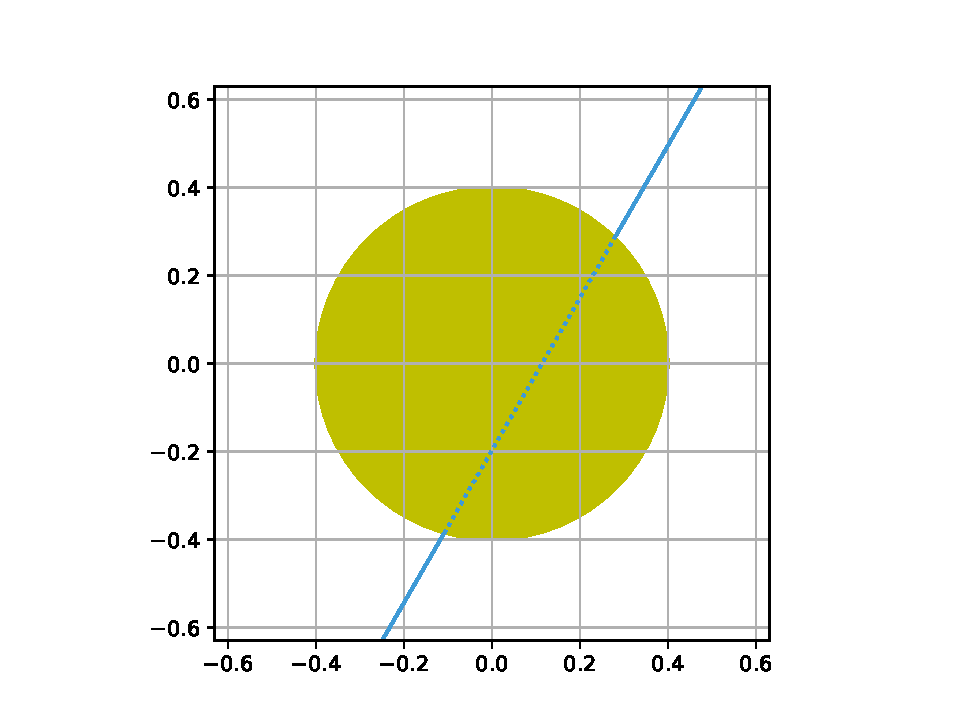
\includegraphics[width=0.67\textwidth]{figs/SingleRay.pdf}
\caption{The Lone Ray}
\label{fig:singleray}
\end{figure}

Let ($x_0$, $y_0$) be the known starting coordinates of the ray--in Fig.~\ref{fig:singleray}, about (-0.25, -0.63) cm. Knowing the geometric parameterse XMIN, XMAX, YMIN, and YMAX and the angle $\varphi$, one can calculate which boundary the ray reaches first. In this example, our ray reaches YMAX first. Therefore, his ending coordinates ($x_1$, $y_1$) will be

\begin{align}\label{eq:x1y1}
x_1 &= x_0 + \frac{\Delta y}{\tan(\varphi)}
\cr
y_1 &= \text{ YMAX}
\end{align}

The next step is to check whether the ray intersects with the fuel pin. Evaluate the following expression for the intersection of a line segment with a circle centered at (0, 0).

\begin{equation}\label{eq:intersection}
R{^\prime}^2 = \frac{ \big[
(x_1 - x_0) y_0 - (y_1 - y_0) x_0
\big]^2 }{ 
(x_1 - x_0)^2 + (y_1 - y_0)^2  }
\end{equation} 

For a perfect cylinder of radius $R$, if $R > R^\prime$, then the ray intersects with the pin. Then, it becomes necesary to determine the exact points where the track enters and exits the pin.

Using the equation for a circle, we can write:

\begin{equation}\label{eq:circler}
x_R^2 + y_R^2 = R^2
\end{equation}

...where the solutions to $x_R$ and $y_R$ represent the locus of points on the edge of the circle.

Let $s_1$ represent the length of the segment of the track before the fuel pin. Then, the coordinates of the first intersection are

\begin{align}\label{eq:xryr}
x_R &= x_0 + s_1 \cos(\varphi)
\cr
y_R &= y_0 + s_1 \sin(\varphi)
\end{align}

Plugging Eq.~\ref{eq:xryr} into Eq.~\ref{eq:circler},

\begin{equation}\label{eq:sone1}
[x_0 + s_1 \cos(\varphi)]^2 + [y_0 + s_1 \sin(\varphi)]^2 = R^2
\end{equation}

...which is a quadratic equation with $s_1$ as the one unknown. Expanding Eq.~\ref{eq:sone1},

\begin{equation}\label{eq:sone2}
[ x_0^2 + 2x_0 s_1 \cos(\varphi) + s_1^2 \cos^2(\varphi) ] + 
[ y_0^2 + 2y_0 s_1 \sin(\varphi) + s_1^2 \sin^2(\varphi) ] = R^2
\end{equation}

Gathering by powers of $s_1$,

\begin{equation}\label{eq:sone3}
[ \cos^2(\varphi) + \sin^2(\varphi) ] \mathbf{s_1^2} + 
2 [ x_0 \sin(\varphi) + y_0 \cos(\varphi) ]  \mathbf{s_1} + 
x_0^2 + y_0^2 - R^2 = 0
\end{equation}

Since $\cos^2(\varphi) + \sin^2(\varphi) = 1$, we can cancel that coefficient before solving the equation for $s_1$ using the quadratic formula.

\begin{equation}\label{eq:s1}
s_1 = \cos(\varphi) x_0 + \sin(\varphi) y_0 +
\sqrt{ R^2 - x_0^2 +
\cos^2(\varphi) [x_0^2 - y_0^2] + 2 \cos(\varphi) \sin(\varphi)}
\end{equation}

For $s_1$, the distance from the starting edge to the fuel pin, the positive solution to the radical is chosen. To find $s_2$, the distance from the pin to the far edge, the negative solution to the radical applies. Both $s_1$ and $s_2$ appear as a solid line in Fig.~\ref{fig:singleray}.

\begin{equation}\label{eq:s2}
s_2 = \cos(\varphi) x_1 + \sin(\varphi) y_1 -
\sqrt{ R^2 - x_1^2 +
\cos^2(\varphi) [x_1^2 - y_1^2] + 2 \cos(\varphi) \sin(\varphi)}
\end{equation}

Of course, the length of the segment going through the fuel pin ($s_f$, the dotted line in Fig.~\ref{fig:singleray}) is just the distance between the starting and ending coordinates, minus the lengths of the segments through the moderator.

\begin{equation}\label{eq:sf}
s_f = \sqrt{(x_1 - x_0)^2 + (y_1 - y_0)^2} - s_1 - s_2
\end{equation}

For tracks that do not intersect the pin, the one segment is of length $\sqrt{(x_1 - x_0)^2 + (y_1 - y_0)^2}$.

\newpage

\subsection{Area Calculations}\label{sec:area}

Recall:

\begin{itemize}
\item From Eq.~\ref{eq:area}, the area of an FSR may be approximated by the summation of the product $w_k s_{k,i}$.
\item From Eq.~\ref{eq:deltavarphi}, effective track width $w_k$ (equivalent to azimuthal track spacing $\delta_\varphi$) can be calculated from the corrected track spacing.
\item From Eqs.~\ref{eq:s1}-\ref{eq:sf}, the lengths of track segments across each FSR are known.
\end{itemize}

Additionally, we know that the sum of the azimuthal quadrature weights over all 4 quadrants must sum to 1. Likewise, the sum of the polar weights over all levels must sum to 1. With this knowledge, we will rewrite Eq.~\ref{eq:area} to include both the azimuthal and polar weights:

\begin{equation}\label{eq:areaquad}
\lim\limits_{N_K \rightarrow \infty} \sum\limits_k^{N_K}
\sum\limits_a^{N_A} \sum\limits_p^{N_P} w_p w_a w_k s_{k,i} = A_i
\end{equation}

In a practical sense, this allows one to calculate the area of an FSR using the following simple algorithm:

\begin{verbatim}
for angle `a' in azimuthal quadrature:
    get `w_a' from quadrature
    for track `k' in tracks:
        w_k = azimuthal spacing 
        s_ki = track.trace()
        for angle `p' in polar quadrature:
            get `w_p' from quadrature
            Area += w_p * w_a * w_k * s_ki
\end{verbatim}

This is useful for testing quadrature implementation and for converging ray spacing. If the appoximated area from Eq.~\ref{eq:areaquad} is sufficiently close to the analytic solution solution for the area, then the quadrature is valid and the ray spacing is probably converged.


\subsection{Flux Calculations}\label{sec:flux}

Each generated track is used twice for flux calculations. First, tracks are followed through all of their reflections in the forward direction (Fig.~\ref{fig:fourtracks}), saving the boundary angular flux to an appropriate index in an array. Then, the same procedure is done for each track in the backward direction, storing flux to a different set of indices in the array. By using the same track for two different angular fluxes ($\varphi$ and $\hat{\varphi}$), the memory requirement for track storage and computational time for ray tracing are halved.

The flux calculation algorithm is similar to that for area calculation. The code iterates over all azimuthal angles, tracks, directions, and polar angles.


\begin{verbatim}
for angle `a' in azimuthal quadrature:
    get `w_a' from quadrature
    for track `k' in tracks:
        for direction `d' in (forward, backward):
            w_k = azimuthal spacing 
           	s1, sf, s2 = track.trace(d)
            for angle `p' in polar quadrature:
                get `w_p' from quadrature
                get `psi_in' from boundary condition
                for each segment `s':
                    get `FSR' that s goes through
                    get `FSR_AREA', `source', `sigma' from FSR
                    attenuation = f(sigma, s)
                    delta_psi = f(psi_in, source, attenuation)
                    psi_out = psi_in - delta_psi
                    scalar_flux += w_p * w_a * w_k * delta_psi / FSR_AREA
                    psi_in = psi_out
                psi[k, d, p] = psi_out
scalar_flux += source
scalar_flux *= 4pi/sigma
\end{verbatim}

The variables \texttt{delta\_psi} and \texttt{scalar\_flux} are calculated according to Eqs.~\ref{eq:deltapsi} and \ref{eq:scalarflux}, respectively. \texttt{psi\_in} corresponds to $\psi_{a,k,i,p}(s_0)$.

The array \texttt{psi[k, d, p]} stores the boundary flux. If reflective boundary conditions apply, the first \texttt{psi\_in} corresponds to the outgoing flux of the track terminating at \texttt{psi[k, d, p]}. Under vacuum boundary conditions, \texttt{psi\_in} is 0.

Convergence is determined by

\begin{itemize}
\item the change in scalar flux in each FSR between iterations:

\begin{equation}\label{eq:fluxdiff}
\epsilon = \frac{|\phi_f^{new} - \phi_f^{old}|}{\phi_f^{new}}
\hspace{1cm} \text{and} \hspace{1cm}
\epsilon = \frac{|\phi_m^{new} - \phi_m^{old}|}{\phi_m^{new}}
\end{equation}
\item  and the L2 engineering norm of the angular flux array:

\begin{equation}\label{eq:l2norm}
\epsilon = 
\sqrt{ \frac{1}{N_K N_P} \sum\limits_k^{N_K} \sum\limits_p^{N_P} 
\left( \frac{\psi_{k, p}^{new} - \psi_{k, p}^{old}}{\psi_{k, p}^{new}} \right)^2 }
\end{equation}
\end{itemize}

For this problem set, the maximum tolerance $\epsilon$ was set to $10^{-5}$ for each of the three convergence criteria.

\newpage
\subsection{Dancoff Factor Calculations}\label{sec:dancoff}

The Dancoff factor $D$ relates the fuel-to-fuel collision probability between isolated rods and infinite arrays.

For an isolated rod, apply Wigner's rational approximation:

\begin{equation}\label{eq:pff0}
P_{f \rightarrow f}^0 = \frac{\ell \Sigma_f}{1 + \ell \Sigma_f}
\end{equation}

...where $\Sigma_f$ is the total macroscopic cross section in the fuel and $\ell$ is the mean chord length. In an infinite cylinder, the mean chord length equals twice the radius ($\ell = 2 R$).

For an infinite lattice, the ratio of probability of neutron ending up in the fuel vs. the moderator can be expressed in terms of the ratio of reaction rates:


\begin{align}\label{eq:rxrates}&
\phi_m A_m \propto \frac{Q}{\Sigma_m} P_{f \rightarrow m}^\infty
\hspace{0.5cm} \text{and} \hspace{0.5cm}
\phi_f A_f \propto \frac{Q}{\Sigma_f} P_{f \rightarrow f}^\infty
\cr \rightarrow &
\frac{\Sigma_m \phi_m A_m}{\Sigma_f \phi_f A_f} = 
\frac{P_{f \rightarrow m}^\infty}{P_{f \rightarrow f}^\infty} = 
\frac{1 - P_{f \rightarrow f}^\infty}{P_{f \rightarrow f}^\infty} = 
\frac{1}{P_{f \rightarrow f}^\infty} - 1
\cr \rightarrow & 
P_{f \rightarrow f}^\infty = \frac{1}{1 + 
\frac{\Sigma_m \phi_m A_m}{\Sigma_f \phi_f A_f} }
\end{align}

The Dancoff correction $C$ is defined as

\begin{equation}\label{eq:d}
C = 1 - D = 1 - \frac{P_{f \rightarrow f}^0}{P_{f \rightarrow f}^\infty}
\end{equation}

...such that a single isolated rod has a Dancoff correction of 0 and a voided lattice has a Dancoff correction of 1.

Alternatively, $C$ may be directly calculated from the MOC using Eq.~\ref{eq:c}.

\begin{equation}\label{eq:c}
C = 1 - \frac{\frac{4\pi Q}{\Sigma_f} - \phi_f^\infty}{\frac{4\pi Q}{\Sigma_f} - \phi_f^0}
\end{equation}

$\phi_f^\infty$ is the flux in the fuel region in the actual lattice, modeled by reflective boundary conditions. The flux in an isolated fuel pin, $\phi_f^0$, may be calculated by imposing vacuum boundary conditions on the geometry and performing a single transport sweep.


\newpage
\section{Results}\label{sec:results}

\subsection*{\ref{sec:results}.0\hspace{10pt} Tests}\label{sec:tests}

Several tests were performed to ensure that the MOC code was performing as expected.

\subsubsection{Ray pattern test}

\begin{figure}[h]
\centering
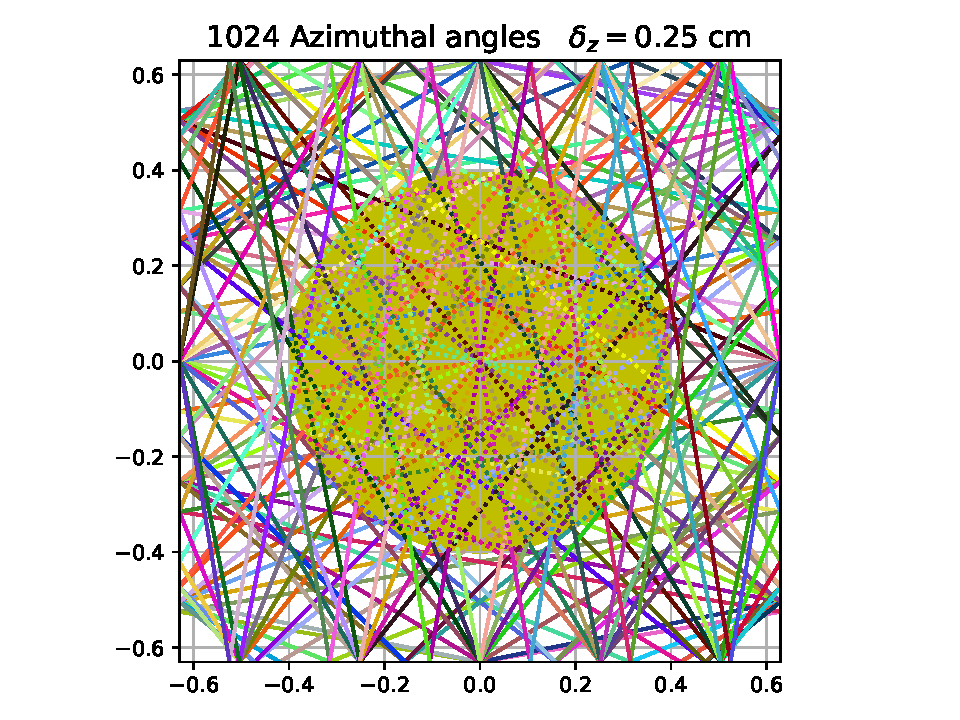
\includegraphics[width=0.67\textwidth]{figs/1024_angles.pdf}
\caption{"Holes" in ray patterns}
\label{fig:holes}
\end{figure}

Given sufficiently fine angular resolution, one should observe "holes" in the track generation pattern. Quarter circles of radius $\delta/2$ should appear at the corners. A sparse circle of the same radius appears in the exact center. Other sparse or empty circles appear in regular intervals over the geometry.

\subsubsection{Cyclic track test}\label{sec:testcyclic}

\begin{figure}[H]
\centering
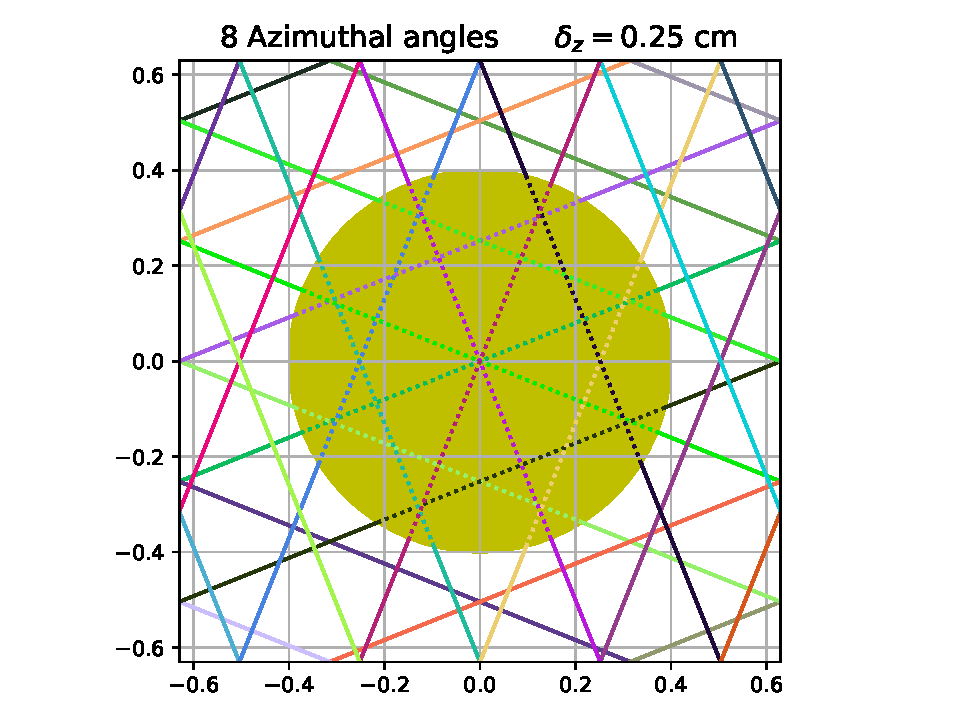
\includegraphics[width=0.67\textwidth]{figs/8_angles.pdf}
\caption{Two complete cycles}
\label{fig:cyclictracks}
\end{figure}

If tracks are properly reflected, they should form complete cycles over the geometry, and their indices in the angular flux array should have a clear progression around each cycle. For the tracks in Fig.~\ref{fig:cyclictracks}, the starting and ending indices and coordinates are printed out below. We see that the tracks of both cycles reflect are properly linked to exactly two others in their cycles, and the last track in each cycle returns to the starting coordinates.

\begin{verbatim}
0  1  (-0.63   0.504)(-0.315  0.63)  | 14  15 (-0.63   0.315)(-0.504  0.63)
1  2  (-0.315  0.63)  (0.63   0.252) | 15  16 (-0.504  0.63)  (0.0  -0.63)
2  3   (0.63   0.252)(-0.63  -0.252) | 16  17  (0.0   -0.63)  (0.504  0.63)
3  4  (-0.63  -0.252) (0.315 -0.63)  | 17  18  (0.504  0.63)  (0.63  0.315)
4  5   (0.315 -0.63)  (0.63  -0.504) | 18  19  (0.63   0.315) (0.252  -0.63)
5  6   (0.63  -0.504)(-0.63   0.0)   | 19  20  (0.252 -0.63) (-0.252  0.63)
6  7  (-0.63   0.0)   (0.63   0.504) | 20  21 (-0.252  0.63) (-0.63  -0.315)
7  8   (0.63   0.504) (0.315  0.63)  | 21  22 (-0.63  -0.315)(-0.504  -0.63)
8  9   (0.315  0.63) (-0.63   0.252) | 22  23 (-0.504 -0.63)  (0.0  0.63)
9  10 (-0.63   0.252) (0.63  -0.252) | 23  24  (0.0    0.63)  (0.504  -0.63)
10 11  (0.63  -0.252)(-0.315 -0.63)  | 24  25  (0.504 -0.63)  (0.63  -0.315)
11 12 (-0.315 -0.63) (-0.63  -0.504) | 25  26  (0.63  -0.315) (0.252  0.63)
12 13 (-0.63  -0.504) (0.63   0.0)   | 26  27  (0.252  0.63) (-0.252  -0.63)
13 0   (0.63   0.0)   (-0.63  0.504) | 27  14 (-0.252 -0.63) (-0.63  0.315)
\end{verbatim}


\newpage
\subsubsection{Area convergence test}\label{sec:testarea}

The MOC solver should be able to estimate the area of the two flat source regions. If the quadrature is valid, as the ray spacing becomes increasingly fine, the estimated area should approach the actual area.

Area calculations with the Tabuchi-Yamamoto quadrature using 1, 2, and 3 levels were performed using 4, 8, 16, and 32 azimuthal angles. As one would expect, the number of polar levels did not affect the area calculation: the 2D projection along the polar angles does not change. Area changed slightly with the number of azimuthal angles, but beyond the coarsest ray spacing, it had little effect. The results tabulated in this section were found using 8 azimuthal angles.

Area calculations were run for track spacing of 0.5, 0.1, 0.05, 0.01, 0.005, and 0.001 cm. The area estimation converged on the order of the desired tolerance with spacing of around 0.001 to 0.005 cm. The relevant results for the area calculation using are below.

$ $

\begin{verbatim}
============================================================
D_AZIM = 0.5 cm
------------------------------------------------------------
Fuel area
    Actual: 0.502655    Effective: 0.552217
    Error: 9.8601%

Moderator area
    Actual: 1.084945    Effective: 1.035383
    Error: 4.5682%

============================================================
D_AZIM = 0.1 cm
------------------------------------------------------------
Fuel area
    Actual: 0.502655    Effective: 0.505257
    Error: 0.5178%

Moderator area
    Actual: 1.084945    Effective: 1.082343
    Error: 0.2399%

============================================================
D_AZIM = 0.05 cm
------------------------------------------------------------
Fuel area
    Actual: 0.502655    Effective: 0.502836
    Error: 0.0361%

Moderator area
    Actual: 1.084945    Effective: 1.084764
    Error: 0.0167%

============================================================
D_AZIM = 0.01 cm
------------------------------------------------------------
Fuel area
    Actual: 0.502655    Effective: 0.502699
    Error: 0.0089%

Moderator area
    Actual: 1.084945    Effective: 1.084901
    Error: 0.0041%

============================================================
D_AZIM = 0.005 cm
------------------------------------------------------------
Fuel area
    Actual: 0.502655    Effective: 0.502661
    Error: 0.0012%

Moderator area
    Actual: 1.084945    Effective: 1.084939
    Error: 0.0005%

============================================================
D_AZIM = 0.001 cm
------------------------------------------------------------
Fuel area
    Actual: 0.502655    Effective: 0.502662
    Error: 0.0014%

Moderator area
    Actual: 1.084945    Effective: 1.084938
    Error: 0.0007%
\end{verbatim}


\newpage
\subsubsection{Flux ratio test}\label{sec:testflux}

The fuel-to-moderator flux ratio should behave predictably with changes to the source and cross section in each flat source region. Several simple tests were created to see if the fluxes changed as expected.

\begin{enumerate}
\item Equal $Q_{FSR}$, $\Sigma$ for both regions. We expect the flux ratio to be exactly 1.0.

\item $Q_{FUEL}$, $\Sigma_f$ double that of (1). We expect the flux ratio to remain exactly 1.0.

\item Double $Q_{FSR}$ for both regions, but same $\Sigma$ as  (1). We expect the individual fluxes to double, and the flux ratio to remain exactly 1.0.

\item Double $Q_{FUEL}$, same $\Sigma$ as in (1), but no source in moderator. We expect to see a higher flux in the fuel than the moderator.

\item $Q_{FUEL}$ and $\Sigma$ same as in (1), but no source in moderator. We expect to see the same flux ratio as (4), with individual fluxes half that of (4).
\end{enumerate}

The expected results were observed in all 5 tests. The raw output is below.

\begin{verbatim}

Cell 1: Fuel XS=1.0, Mod XS=1.0, Qfuel=1.0, Qmodr=1.0
    Fuel flux: 1.0000    Mod flux: 1.0000
    Fuel-to-mod flux ratio: 1.000

Cell 2: Fuel XS=2.0, Mod XS=1.0, Qfuel=2.0, Qmodr=1.0
    Fuel flux: 1.0000    Mod flux: 1.0000
    Fuel-to-mod flux ratio: 1.000

Cell 3: Fuel XS=1.0, Mod XS=1.0, Qfuel=2.0, Qmodr=2.0
    Fuel flux: 2.0000    Mod flux: 2.0000
    Fuel-to-mod flux ratio: 1.000

Cell 4: Fuel XS=1.0, Mod XS=1.0, Qfuel=2.0, Qmodr=0.0
    Fuel flux: 0.93899    Mod flux: 0.49157
    Fuel-to-mod flux ratio: 1.910

Cell 5: Fuel XS=1.0, Mod XS=1.0, Qfuel=1.0, Qmodr=0.0
    Fuel flux: 0.46950    Mod flux: 0.24578
    Fuel-to-mod flux ratio: 1.910
\end{verbatim}


\newpage
\subsection{Flux Ratios}\label{sec:fluxratios}

\begin{itemize}
\item Write an MOC program that edits one-group volume-averaged fluxes in fuel and coolant, given a spatially uniform, isotropic source in the fuel having a pure removal cross section (= potential scatter) and coolant with pure absorption cross section = [0.0, 0.25, 1.0, 5.0, and $\infty$] cm$^{-1}$.
\end{itemize}

\subsubsection{Cross Sections}\label{sec:crosssections}

The macroscopic fuel cross section is calculated from the microscopic cross sections.

\begin{align}\label{eq:macrofuel}
& \Sigma_f = N_{238} * \left( \sigma_{p,U238} + 2 \sigma_{p,O16} \right) =
\cr \rightarrow
& \Sigma_f = 0.022 \times 10^{24} \frac{\text{at}}{\text{ cm}^3} * 
\left( 11.4 + 2*4.0  \right) \times 10^{-24} \text{ cm}^2/\text{at}
\cr \rightarrow
& \Sigma_f = 0.4268 \text{ cm}^{-1}
\end{align}

In order to avoid NaNs, the 0.0 cm$^{-1}$ coolant cross section has been replaced with a value of $10^{-6} \text{ cm}^{-1}$ (an order of magnitude below the numerical tolerance), and the infinite cross has been replaced with $10^{6} \text{ cm}^{-1}$. (The code would still run with 0 and $\infty$ cross sections, but the flux ratios or convergence criteria would be NaN.)

\subsubsection{Angular Convergence}\label{sec:angularconvergence}

To converge the solution in number of angles, flux calculations were performed with increasing numbers of azimuthal angles. Results have been tabulated below for target azimuthal spacings of $\delta_\varphi$ = 0.005 and 0.001 cm, which were considered to be converged according to Section~\ref{sec:testarea}, as well as $\delta_\varphi = 0.0001$ cm for good measure. The first nonzero moderator cross section ($\Sigma_m = 0.25\text{ cm}^{-1}$) was used.

\begin{table}[H]
\centering
\caption{$\delta_\varphi = 0.005$ cm}
\label{tab:dazim0050}
\begin{tabular}{c|c|r}
\hline
N\_Azim & Flux Ratio & \% Change \\
 \hline \hline
4	&	1.35933	&	------ \hspace{6pt}	\\
8	&	1.08595	&	20.111\%	\\
16	&	1.12452	&	3.551\%	\\
32	&	1.17393	&	4.394\%	\\
64	&	1.20018	&	2.236\%	\\
128	&	1.20570	&	0.459\%	\\
256	&	1.20626	&	0.047\%	\\
512	&	1.20642	&	0.013\%	\\
1024	&	1.20644	&	0.002\%	
\end{tabular}
\end{table}


\begin{table}[H]
\centering
\caption{$\delta_\varphi = 0.001$ cm}
\label{tab:dazim0010}
\begin{tabular}{c|c|r}
\hline
N\_Azim & Flux Ratio & \% Change \\
 \hline \hline
4	&	1.35929	&	------ \hspace{6pt}	\\
8	&	1.08595	&	20.108\%	\\
16	&	1.12452	&	3.551\%	\\
32	&	1.17402	&	4.402\%	\\
64	&	1.20025	&	2.234\%	\\
128	&	1.20572	&	0.455\%	\\
256	&	1.20622	&	0.042\%	\\
512	&	1.20641	&	0.016\% 
\end{tabular}
\end{table}

\begin{table}[H]
\centering
\caption{$\delta_\varphi = 0.0001$ cm}
\label{tab:dazim0001}
\begin{tabular}{c|c|r}
\hline
N\_Azim & Flux Ratio & \% Change \\
 \hline \hline
4	&	1.35935	&	------ \hspace{6pt}	\\
8	&	1.08596	&	20.112\%  \\
16	&	1.12454	&	3.553\%	  \\
32	&	1.17417	&	4.413\%	  \\
64	&	1.20025	&	2.221\%	  \\
128	&	1.20572	&	0.456\%	  \\
256	&	1.20626	&	0.045\%	  \\
512	&	1.20643	&	0.014\%	
\end{tabular}
\end{table}

For purposes of this problem set, 256 azimuthal angles were selected. The change in the flux ratio beyond 256 angles was on the order of $0.01\%$ in every case.

\begin{figure}[H]
\centering
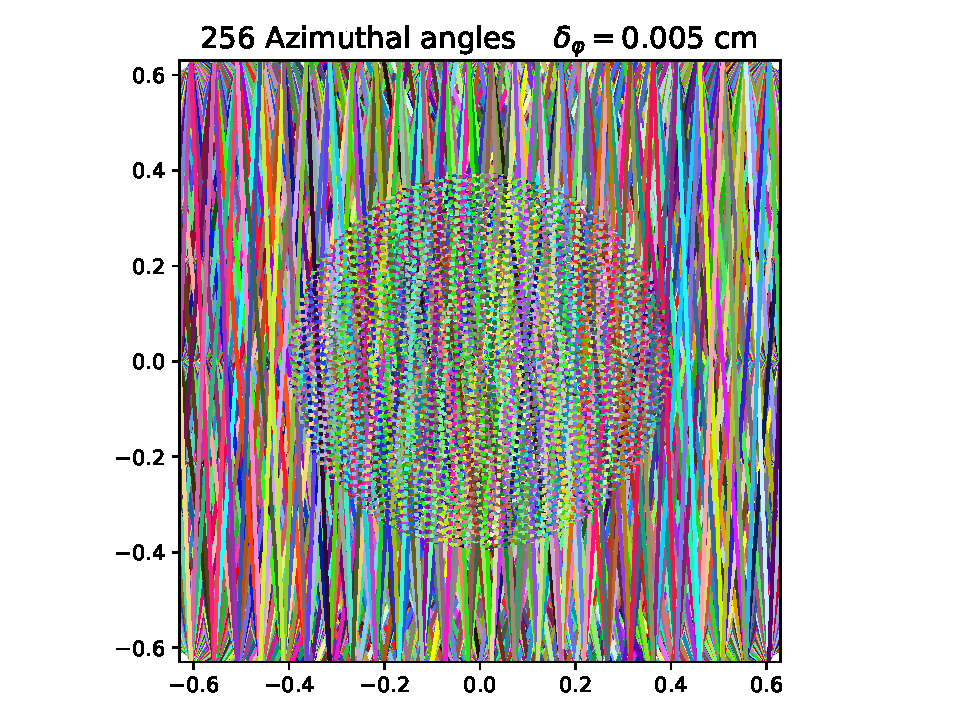
\includegraphics[width=0.6\textwidth]{figs/Converged.pdf}
\caption{Rays converged in space and angle}
\label{fig:converged}
\end{figure}

The TY3 quadrature was used for polar angle discretization. Due to the availability of weights and thetas for only 1, 2, or 3 polar angles in the Tabuchi-Yamamoto quadrature (Fig.~\ref{fig:tylo}), the TY3 solution was considered to be converged in polar angle.


\subsubsection{Flux Ratio Results}\label{sec:fluxratioresults}

\begin{table}[H]
\centering
\caption{Fuel-to-moderator flux ratio, \\ 256 Azimuthal Angles, 3 Polar Angles}
\label{tab:prob1}
\begin{tabular}{c|c|c}
\hline
$\Sigma_m$ & Flux Ratio   & Flux Ratio \\
(cm$^{-1}$) & ($\delta_\varphi = 0.005$ cm) & 
($\delta_\varphi = 0.001$ cm) \\
 \hline \hline
$10^{-6}$	&	1.00003	&	1.00000\\
0.25	 	&	1.20564	&	1.20622\\
1.00		&	1.83543	&	1.83596\\
5.00		&	5.75756	&	5.75976\\
$10^6$		&	$1.122\times10^6$	&	$1.123\times10^6$	\\
\end{tabular}
\end{table}

\subsection{Dancoff Factors}\label{sec:dancofffactoresults}

\begin{itemize}
\item Make a Table of Dancoff factors ($\Sigma_f = 1000.0 \text{ cm}^{-1}$) and $P_{f \rightarrow f} $ vs. coolant cross section
\end{itemize}

A ray spacing of $\delta_\varphi = 0.005 \text{ cm}^{-1}$ and 256 Azimuthal angles were used for the flux calculations. Eq.~\ref{eq:pff0} and Fig.~\ref{fig:hebert} (below) were applied to check the values of $P_{f \rightarrow f}$ and $C$ as determined by the MOC code. 

$ $

\begin{figure}[h]
\centering
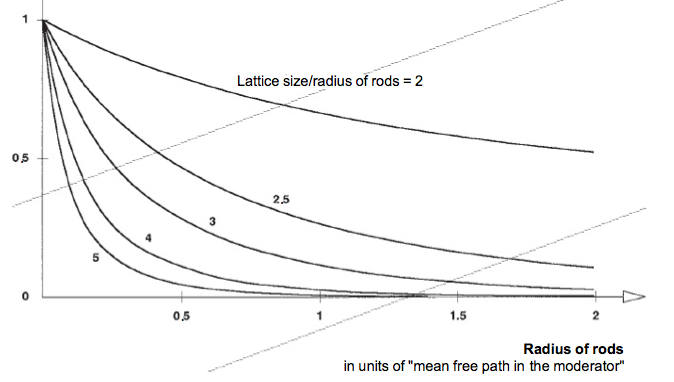
\includegraphics[width=0.67\textwidth]{figs/Graph.png}
\caption{Dancoff Correction reference values \\
Lattice size/radius of rods = 3.15}
\label{fig:hebert}
\end{figure}

\begin{table}[H]
\centering
\caption{Collision probabilities and Dancoff factors}
\label{tab:prob2}
\begin{tabular}{c|c|c|c|c|c|c}
\hline
& & & & &\\
$\Sigma_m$ (cm$^{-1}$) & Flux ratio &
$P_{f \rightarrow f}^\text{Wigner}$ &
$P_{f \rightarrow f}^\text{MOC}$ &
$C$ (Fig.~\ref{fig:hebert}) & 
$C$ (MOC) & $D$ \\
	\hline \hline
$10^{-6}$	&	1.00003	&			&	1.00000	&	1		&	1.00000	&	0.00000	\\
0.25		&	1.40082	&			&	0.99996	&	0.7		&	0.69203	&	0.30797	\\
1.00		&	2.48096	&	0.99988	&	0.99991	&	0.3		&	0.30449	&	0.69551	\\
5.00		&	8.78049	&  &	0.99988	& $< 0.1$\hspace{12pt}	&	0.01744	&	0.98256	\\
$10^6$		& $1.73\times10^6$	&	&	0.99987	&	0	&	0.00000	&	1.00000	\\
\end{tabular}
\end{table}

\section{Conclusions}\label{sec:conclusions}

\begin{itemize}
\item A successful ray tracer was developed for the geometry present in this problem set. 
To make generalize it, the \texttt{Ray()} and \texttt{Cell()} classes would need to be expanded to model general quadratic surfaces, not necessarily a single cylinder. (Section~\ref{sec:raytracing})

\item Reflective boundary conditions were applied through the use of cyclic tracks, which indexed to an array of the angular flux on the boundary. (Section~\ref{sec:testcyclic})

\item Area calculations were converged in ray spacing. The effective area of the flat source regions matched the analytic solution for the area within tolerance. (Section~\ref{sec:testarea})

\item Fuel and moderator fluxes behaved as expected for changes to the source strength and macroscopic cross sections. (Section~\ref{sec:testflux})

\item Flux ratios were converged in angle. (Section~\ref{sec:angularconvergence})

\item Flux ratios were calculated using the converged tracks. For a near-0 moderator cross section, fuel and moderator flux was essentially equal. This makes sense intuitively, as the source was only in the fuel and there was no loss of particles in the moderator. As the moderator cross section increased (with the fuel unchanged), the fuel-to-moderator flux ratio increased. At a "very high" moderator cross section, the fuel-to-moderator flux ratio was effectively infinite. (Section~\ref{sec:fluxratioresults})

\item Dancoff factors and fuel-to-fuel collision probabilities were also calculated. With a near-0 moderator cross section, the problem modeled a voided lattice. $P_{f \rightarrow f}$ was 1, and the Dancoff correction $C$ was 1. As the moderator cross section was increased, $P_{f \rightarrow f}$ began to approach the value predicted by the Wigner Rational Approximation for an isolated pincell within numerical tolerance ($\epsilon = 10^{-5}$), and the Dancoff correction fell to 0. In all cases, $C$ was as close to the value predicted by Fig.~\ref{fig:hebert} as the image resolution allowed. (Section~\ref{sec:dancofffactoresults})

\end{itemize}

\end{document}
